%--------------------------------------------------------------------------------------------------
\chapter{Heterogeneous Streaming Sources Data Fusion for Machine Learning}
\label{ch:data-fusion}
%--------------------------------------------------------------------------------------------------

\epigraph{Data fusion is like a marriage: integrating data sources together requires patience, compromise, and a common language.}{\textit{Kirk Borne}}

% anouncing the paper
\begin{quote}
This chapter presents the paper titled \textit{Streaming data fusion for the internet of things} by Klemen Kenda, Blaž Kažič, Erik Novak and Dunja Mladenić and presents the centerpiece of this thesis. The paper was published in the Sensors journal \cite{kenda:2019:fusion}.
Klemen Kenda is the main author of the paper. 
He contributed to conceptualization, methodology, software development, validation, formal analysis, data curation, writing, visualization, project administration and funding acquisition.
\end{quote}

% introduction
In the context of the Internet of Things (IoT), data fusion, also known as sensor data fusion or information fusion, refers to the process of combining and integrating data from multiple sensors or sources to create a more accurate, comprehensive, and meaningful representation of the environment or system being monitored. 

The main goal of data fusion in IoT is to extract valuable insights, improve decision-making, and enhance the overall efficiency of IoT applications. 
By fusing data from multiple sensors, the resulting information can provide a more accurate understanding of the environment, which can result in better modeling capabilities such as creating predictions or anomaly detection, and a more holistic view of the system's behavior. 

%\highlight{Role of semantic fusion?}
There are several types of data fusion techniques used in IoT, that vary from local to more global approaches and are based on the JDL model \cite{hall:2001:multisensor}:
\begin{enumerate}
    \item \textbf{Sensor-level Fusion:} This involves combining raw sensor data at the individual sensor level to reduce noise and errors. It can include techniques like filtering, calibration, and data alignment.
    
    \item \textbf{Feature-level Fusion:} In this approach, extracted features from the data of different sensors are combined to create a more informative representation. This can help in reducing data dimensionality and improving the efficiency of analysis.
    
    \item \textbf{Decision-level Fusion:} Here, the outputs or decisions from multiple sensors are combined to make a more reliable decision. This technique is often used to improve accuracy and robustness in applications like object tracking or localization.
    
    \item \textbf{Information-level Fusion:} This is the highest level of fusion, where higher-level knowledge or context is integrated into the data to create a comprehensive understanding of the situation. This can involve incorporating external data sources, historical data, or expert knowledge.
\end{enumerate}

% introduction to paper
Our methodology focuses on feature-level fusion and is ignorant of any high-level semantic information regarding the observed system, such as sensor metadata or even system's knowledge graph \cite{kenda:2019:fusion}. 
The goal of the research was to create a useful component in the lambda architecture that would enable fast deployment of real-world IoT applications of machine learning, such as predictive modeling or anomaly detection.

% methodology
The paper provides a formal definition of heterogeneous data streams fusion, a working streaming data fusion framework and conceptual architecture of the system.
In the lambda architecture, the data fusion component is located immediately after data cleaning (see Figure \ref{fig:the_big_picture}).

The methodology is able to ingest 3 types of data: streaming sensor data, updating predictions (such as weather forecasts) and static data (such as data describing human behaviour, for example working days).
Three algorithms are presented that enable the framework to generate enriched data streams and fuse them locally and globally.

% evaluation
The system has been deployed both in a cloud environment and on an edge device. 
Validation of the methodology's efficiency has been accomplished through cloud deployment, using public train data from edge devices on the smart-grid dataset. Additionally, performance evaluation was conducted on the traffic dataset.

The findings strongly support the advantages of employing data fusion techniques. Enhanced data streams have demonstrated a higher model accuracy when compared to non-enriched streams. Moreover, the utilization of multiple data streams that provide contextual information has yielded superior model outcomes in comparison to relying solely on single-source data streams.

The implemented system has been successfully deployed across two distinct environments: a cloud-based infrastructure and an edge computing device.
In a cloud-based deployment, the methodology's efficiency has been validated on the smart-grid dataset. 
On the edge devices, deployed in electric public trains, the methodology's effectiveness has been validated on the traffic dataset.

The results confirm the benefits of using data fusion methods: enriched data streams yield better model accuracy than non-enriched and streams from multiple data streams that describe more context yield better model results than single source data streams.
Additional validation of the overall system water management scenarios is given also in Chapter \ref{ch:big_data_framework}.

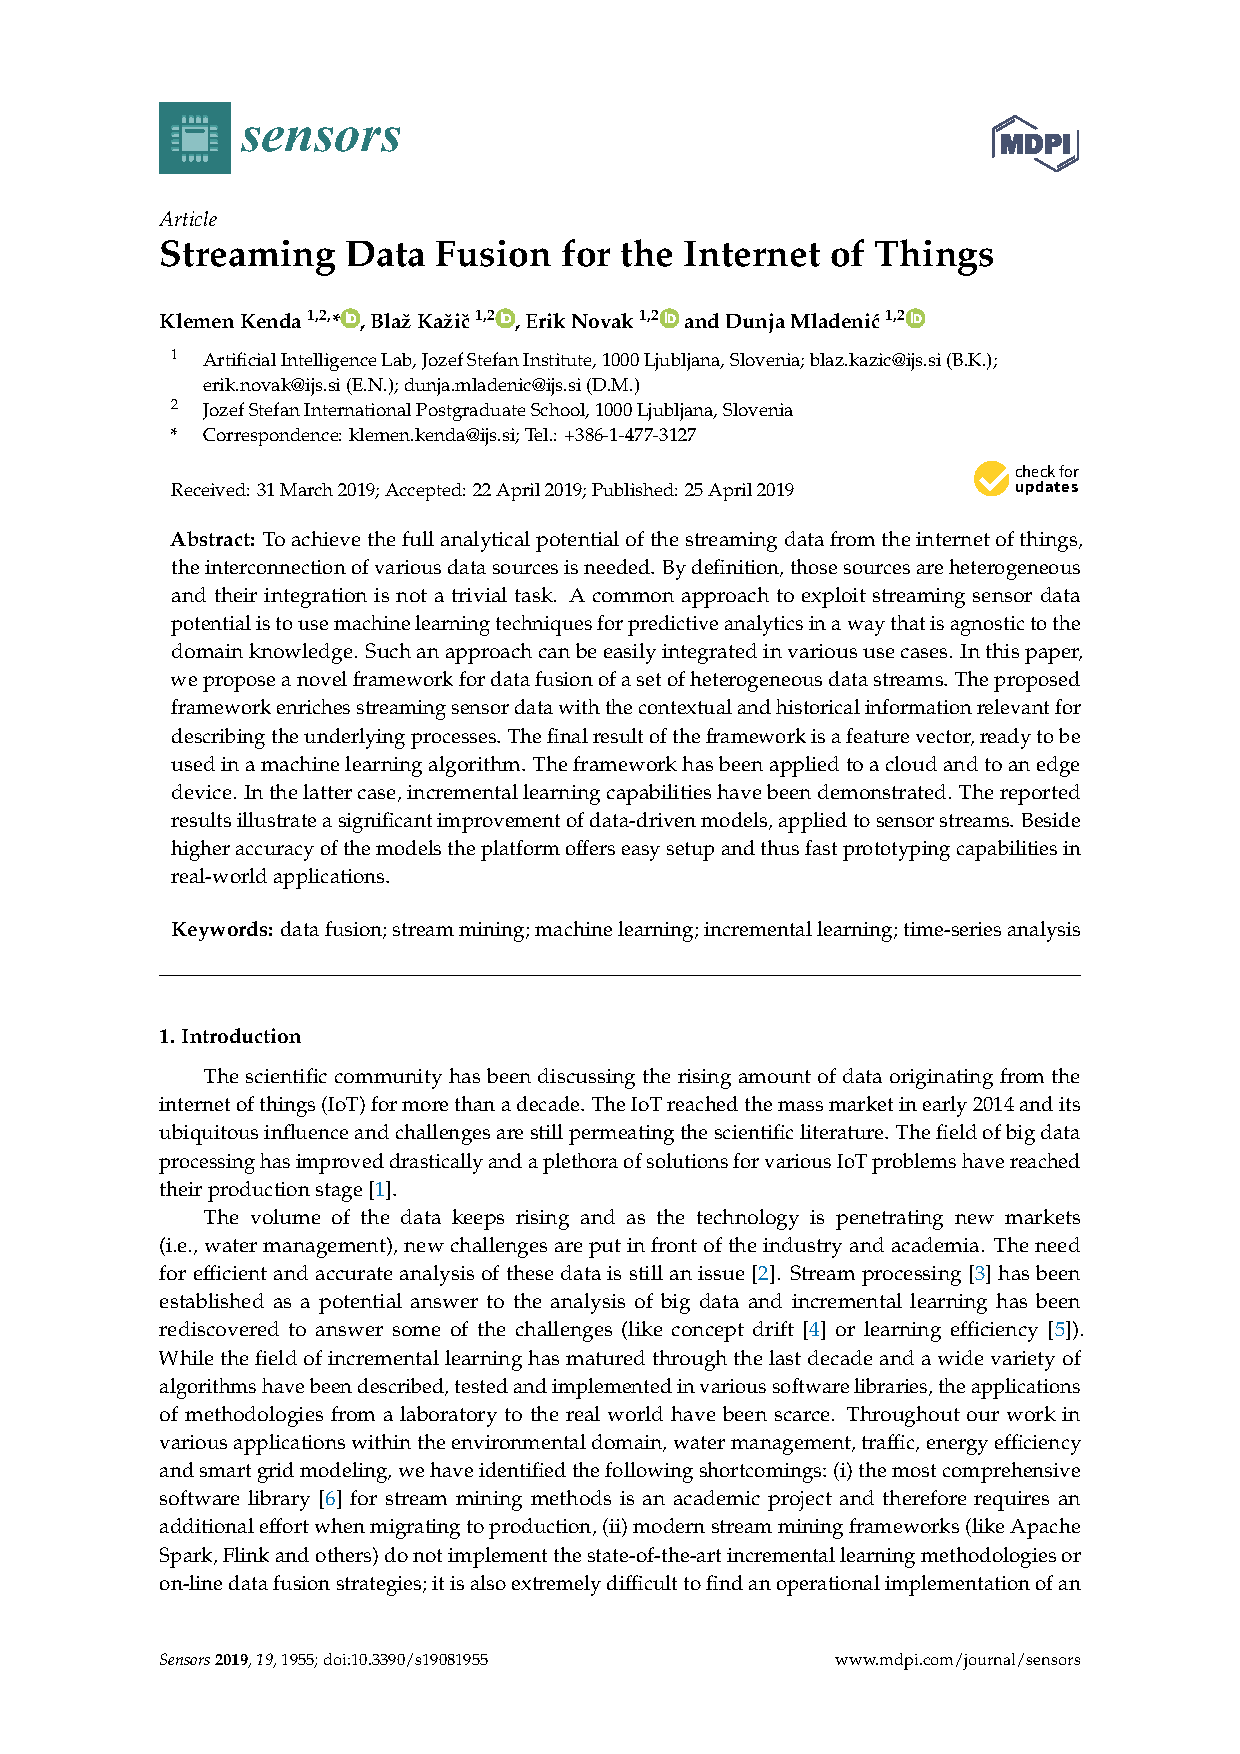
\includepdf[pages=-]{papers/streaming_data_fusion_for_iot.pdf}